% Compile using: TEXINPUTS=minted/source: xelatex -shell-escape slides.tex
\documentclass[12pt,compress,english,utf8,t]{beamer}

\usepackage{etex}

\usepackage[english]{babel}

\usepackage{tikz}
\usepackage{booktabs}
\usepackage{ragged2e}

\usepackage{minted}
\setminted{linenos}

\usepackage[protrusion=true,expansion=false]{microtype}

\title[Pugs, an experimental Perl 6 platform: a retrospective]{A retrospective on Pugs}
\author[Augsburg.pm]{
  \vspace{-0.5em} \\
  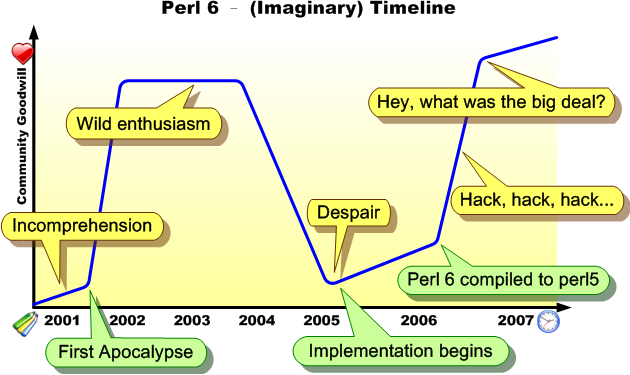
\includegraphics[scale=0.35]{images/timeline} \\[0.8em]
  Ingo Blechschmidt \\
  \small \texttt{<iblech@web.de>} \\
  {\scriptsize March ??th, 2015}
}
\date{March ??th, 2015}

\usetheme{Warsaw}
\usecolortheme{seahorse}
\definecolor{mypurple}{RGB}{60,0,255}  % Audrey's personal blog color, with full saturation
\setbeamercolor{structure}{fg=mypurple}
\usefonttheme{serif}
\usepackage{mathpazo}
\useinnertheme{rectangles}
\setbeamercovered{invisible}

\setbeamertemplate{title page}[default][colsep=-1bp,rounded=false,shadow=false,bg=white]
\setbeamertemplate{frametitle}[default][colsep=-2bp,rounded=false,shadow=false,center]

\setbeamertemplate{navigation symbols}{}
\setbeamertemplate{headline}{}

\newcommand*\oldmacro{}%
\let\oldmacro\insertshorttitle%
\renewcommand*\insertshorttitle{%
  \oldmacro\hfill\insertframenumber\,/\,\inserttotalframenumber\hfill}

\newcommand{\hil}[1]{{\usebeamercolor[fg]{item}{\textbf{#1}}}}

\newcommand{\atpos}[4]{%
  \begin{tikzpicture}[remember picture, overlay]%
    \node[anchor=south east] at (current page.south east) {#1};
  \end{tikzpicture}%
}

\newcommand{\centeredpar}[1]{%
  \begin{center}
    \parbox{0.9\textwidth}{%
      #1%
    }%
  \end{center}%
}

\newcommand{\sourcedquote}[4]{%
  ``#1''\par%
  {\raggedleft -- #2, #3, \href{#4}{link}\par}%
}

% Gonzalo Medina, http://tex.stackexchange.com/a/228198
\makeatletter
\def\Mdescription#1{%
  \advance\beamer@descdefault by \labelsep%
  \list
  {}
  {\labelwidth\beamer@descdefault%
  \leftmargin\beamer@descdefault%
  \let\makelabel\beamer@descriptionitem
  \settowidth\labelwidth{\beamer@descriptionitem{#1}}%
  \setlength\leftmargin{\labelwidth}% 
  \addtolength\leftmargin{\labelsep}%
  }%
  \beamer@cramped%
  \raggedright
  \beamer@firstlineitemizeunskip%
}
\def\endMdescription{\ifhmode\unskip\fi\endlist}
\long\def\beamer@descriptionitem#1{%
  \def\insertdescriptionitem{#1}%
  {\usebeamertemplate**{description item}}\hfil}
\makeatother

\setbeameroption{show notes}

\begin{document}

\frame{\titlepage}

\frame[plain]{
  \centeredpar{
    \justifying\scriptsize
    \textbf{Abstract.}
    ``Hi. Today I have started working on specifying and implementing
    Featherweight Perl 6 (FP6), a side-effect-free subset of Perl~6.''
    Audrey Tang used these words to unveil the Pugs project in February of 2005.
    Initially conceived as an implementation of a small subset of Perl~6 in
    Haskell, the project quickly grew to contain a full-fledged compiler and
    interpreter for Perl~6 and attracted a large and diverse community.

    \medskip
    The talk will give a subjective survey of the history of Pugs. We will pay
    particular attention to the special manner with which Audrey Tang led the project and
    what the philosophy ``-Ofun'' meant to the developers. We'll also discuss
    which parts of Pugs were absorbed into other implementations of Perl~6 and
    which influence Pugs had on the Perl and Haskell communities.
    \medskip

    \textbf{Warning.} The account is mostly from memory and not properly
    researched. Try not to trust it! Also note that \emph{the code excerpts are
    edited for legibility}, i.\,e.\@ shortened at a few places.
    \par
  }
}

\frame{\tableofcontents}


\section{Timeline of Pugs development}

\subsection{The beginning}

\logo{
\includegraphics[scale=0.13]{images/audreyt2.jpeg}}
\begin{frame}\frametitle{The beginning}
  \centeredpar{
    \hil{``Hi. Today I have started working on specifying and implementing
    Featherweight Perl 6 (FP6), a side-effect-free subset of Perl~6.''}

    \raggedleft -- Audrey Tang, February 2nd, 2005
  }

  \begin{Mdescription}{2001}
    \item[2001] Apocalypse 1, first Perl 6 design document
    \item[2004] Many Apocalypse and Synopse documents
    \item[2005] Active discussion on perl6-language@perl.org
    \item[2005] Pugs, providing the first implementation
    \item[]
    \item[2005] Facebook
    \item[2005] YouTube
    \item[2008] GitHub
  \end{Mdescription}
\end{frame}
\logo{}

% http://wayback.archive.org/web/20050209100505/http://haskell.org/hawiki/Perl6UsersGolfingSystem
\begin{frame}[fragile]\frametitle{Screenshot}\scriptsize
  \vspace{-2.0em}
  \begin{verbatim}.=====. __  __  ____   ___    _________________________________________
||   || ||  || ||  || ||__'   Pugs 6: Based on the Perl 6 Synopses
||====' ||__|| ||__||  __||   Copyright (c) 2005 Autrijus Tang
||      `===='  ___|| `==='   World Wide Web: http://autrijus.org/pugs
||             `===='         Report bugs to: autrijus@autrijus.org
==           Version: 6.0.0   =========================================

Welcome to Pugs -- Perl6 User's Golfing System
Type :h for help

pugs> :h
Commands available from the prompt:
:h              = show this help message
:q              = quit
. <exp>         = show the syntax tree of an expression
? <exp>         = evaluate an expression

pugs> . ('1' & "2") * ( 3.0 | "4abcd" )
Op2 "*" (Op2 "|" (Val (VStr "1")) (Val (VStr "2"))) (Op2 "&" (Val (VNum 3.0)) (Val (VStr "4abcd")))

pugs> ('1' & "2") * ( 3.0 | "4abcd" )
((3.0 | 4.0) & (6.0 | 8.0))

pugs> :q
Leaving pugs.\end{verbatim}
\end{frame}

\note{
  \begin{itemize}
    \justifying
    \item \sourcedquote{As I'm finding my way through TaPL and ATTaPL today, it occurs to me that
    I should implement a real language as an exercise; that real language turns
    out to be Perl~6. So it begins \ldots}{Audrey Tang}{February 1st,
    2005}{http://wayback.archive.org/web/20050206202119/http://use.perl.org/~autrijus/journal/}
    \item TaPL refers to \emph{Types and Programming Languages}, a
    computer-science book on implementing programming languages.
    \item Actually, there was an implementation before Pugs. Namely, a small
    project sitting in the Parrot source tree.
  \end{itemize}
}


\subsection{The early days}

\begin{frame}[fragile]\frametitle{The early days}
  \begin{Mdescription}{Day 00}
    \item<1-2|only@1-2>[Day 4] ``Parsec; 90\,\% of operators implemented!''

    % https://github.com/audreyt/pugs/blob/e760c8600350603c10c825caf17ca5ce1e2846ae/src/Parser.hs
    % https://github.com/audreyt/pugs/blob/e760c8600350603c10c825caf17ca5ce1e2846ae/src/Prim.hs
    \only<1>{
      \inputminted{haskell}{code-snippets/day4-ast.hs}
    }

    \only<2>{
      \inputminted{haskell}{code-snippets/day4-parser.hs}
      \bigskip
      \inputminted{haskell}{code-snippets/day4-prim.hs}
    }

    \item<3|only@3>[Day 8] ``Pugs 6.0.2; Turing Completeness''

    % https://github.com/audreyt/pugs/blob/e760c8600350603c10c825caf17ca5ce1e2846ae/src/Eval.hs
    User-defined subroutines, variable binding, \ldots\par
    \inputminted{haskell}{code-snippets/day8-eval.hs}

    \item<4|only@4>[Day 12] ``Refactoring''

    eval(), rand(), \ldots\par
    \inputminted{haskell}{code-snippets/day12-prim.hs}

    \item<5|only@5>[Day 13] ``Continuations''

    \inputminted{haskell}{code-snippets/day13-monads.hs}
    \bigskip
    \inputminted{haskell}{code-snippets/day13-ast.hs}

    \item<6|only@6>[Day 14] ``All tests successful''

    \inputminted{perl}{code-snippets/day14-basic.pl}

    \item<7|only@7>[Day 20] ``6.0.8''

    Hashes, pairs, many IO primitives, \ldots\par
    \inputminted{perl}{code-snippets/day20-ycombinator.pl}

    \item<8|only@8>[Day 23] ``Test.pm flies!''

    First Perl 6 module, more than 400 unit tests, \ldots\par
    \inputminted{perl}{code-snippets/day23-test.pm}
  \end{Mdescription}
\end{frame}


\subsection{Further highlights}

\begin{frame}[label=further-highlights]\frametitle{Further highlights}
  \begin{Mdescription}{Tag 00}
    \item[Day 47] ``Perl 5 regular expressions landed.''
    \hyperlink{perl5re}{\beamerbutton{see code}}

    \item[Day 50] Compiling to Parrot

    \item[Day 85] BEGIN blocks
    \hyperlink{begin-blocks}{\beamerbutton{see code}}

    \item[Day 87] ``STM: Atomic power!''
    \hyperlink{stm}{\beamerbutton{see code}}
  \end{Mdescription}
\end{frame}

% Finished http://pugs.blogs.com/pugs/2005/04/page/2/.

\appendix

\section{Day 47: ``Perl 5 regular expressions landed.''}

\begin{frame}[label=perl5re]\frametitle{Day 47: ``Perl 5 regular expressions landed.''}
  \inputminted{text}{code-snippets/day47-regex.pl}

  \hyperlink{further-highlights}{\beamerbutton{Continue slides \ldots}}
\end{frame}

\section{Day 85: BEGIN blocks}

\begin{frame}[label=begin-blocks]\frametitle{Day 85: BEGIN blocks}
  \inputminted{haskell}{code-snippets/day85-parser.hs}

  \hyperlink{further-highlights}{\beamerbutton{Continue slides \ldots}}
\end{frame}

\section{Day 87: ``STM: Atomic power!''}

\begin{frame}[label=stm]\frametitle{Day 87: ``STM: Atomic power!''}
  \inputminted{perl}{code-snippets/day87-atomic.pl}

  \hyperlink{further-highlights}{\beamerbutton{Continue slides \ldots}}
\end{frame}

\note{
  \begin{itemize}
    \justifying
    \item \sourcedquote{One of my goals of this project is to keep it dual-cultured. So the
    source tree is managed with bth svk and darcs; the build system requires
    both Perl5 and GHC; I will submit my Apocrypha series of design documents
    as monthly articles to both Perl.com and The Monad Reader; the project info
    is on both CPAN and the Haskell Wiki; etc, etc.}{Audrey Tang}{February 6st,
    2005}{http://wayback.archive.org/web/20050206202119/http://use.perl.org/~autrijus/journal/}

    \item Foreshadowing node.js:
    \sourcedquote{Indeed, if JavaScript2 does survive the standardization
    process, it is entirely possible that it may become the next Ruby, because
    writing programs that runs at both client and server side is a strong
    motivation -- the same reason to keep Pugs targetable to multiple
    backends.}{Audrey Tang}{October 30th,
    2005}{http://wayback.archive.org/web/20060924085336/http://use.perl.org/journal.pl?op=display&uid=1505&start=10}

    \item \sourcedquote{In other news, Pugs was mentioned on The Haskell
    Sequence today. Indeed, I have noted that a significant part of questions
    asked in \#haskell are from camelfolks. Conversely, we saw a large influx
    from lambdafolks to \#perl6 as well. Lots of knowledge transfer is
    happening, which makes me really happy.}{Audrey Tang}{February 24th,
    2005}{http://pugs.blogs.com/pugs/2005/02/day_24_an_amazi.html}
  \end{itemize}
}

\end{document}

\begin{itemize}
  \item Audrey's first post contained a language semantics question.
  \item Important insight: Specification and implementation have to be
  developed hand in hand.
\end{itemize}

http://www.slideshare.net/autang/pugs-a-perl-6-implementation
http://www.slideshare.net/autang/ofun-optimizing-for-fun
http://perlmonks.org/?node_id=835731

pioneering techniques:
GADTs

fun:
slides "Perl 6, genau jetzt!"

porting modules
testing stuff
force_todo
some builtins
IRC library and bots
hyper operators
state/FIRST
macros
smokeserver
PIL2JS
